\subsection{Chapter 21 - Sources of magnetic field}

\subsubsection{Overview}\label{chapter:magneticsource}

\begin{verbatim}
print("Here is a Python cell")
\end{verbatim}

\begin{verbatim}
print("Another code cell with a second optional metadata syntax")
\end{verbatim}

In this chapter, we develop the tools to model the magnetic field that is produced by an electric current. We will introduce the Biot-Savart Law, which is analoguous to Coulomb's Law in that it can be used to calculate the magnetic field produced by any current. We will also introduce Ampère's Law, which can be thought of as the analogue to Gauss' Law, allowing us to easily determine the magnetic field when there is a high degree of symmetry.

\begin{framed}
\textbf{Learning Objectives}\\
\begin{itemize}
\item Understand how to apply the Biot-Savart Law to determine the magnetic field from an electric current.
\item Understand how to apply Ampère's Law.
\item Understand how to model the forces that are exerted on each other by two wires carrying current.
\item Understand how to model a solenoid and a toroid.
\end{itemize}
\end{framed}

\begin{framed}
\textbf{Think About It}\\
How does an electromagnet work?

\begin{enumerate}
\item Current is passed through a magnet, increasing its strength.
\item Current is passed through a circular coil, creating a magnetic field.
\end{enumerate}

\begin{framed}
\textbf{Answer}\\
\begin{enumerate}[resume]
\item
\end{enumerate}
\end{framed}
\end{framed}

\subsubsection{The Biot-Savart Law}

The Biot-Savart law allows us to determine the magnetic field at some position in space that is due to an electric current. More precisely, the Biot-Savart law allows us to calculate the infinitesimal magnetic field, $d\vec B$, that is produced by a small section of wire, $d\vec l$, carrying a current, $I$, such that $d\vec l$ is co-linear with the wire and points in the direction of the electric current:
\begin{equation}
\boxed{d\vec B = \frac{\mu_0 I}{4\pi}\frac{d\vec l\times \hat r}{r^2}}
\end{equation}
where $\vec r$ is the vector from the element of wire, $d\vec l$, to the point where we would like to determine the magnetic field, as illustrated in Figure~\ref{fig:magneticsource:biotsavart}. $\mu_0$ is a constant of proportionality called the ``permeability of free space'', and has the value $\mu_0=4\pi \times 10^{ -7} {\rm T\cdot m/A}$.

\begin{figure}[!htbp]
\centering
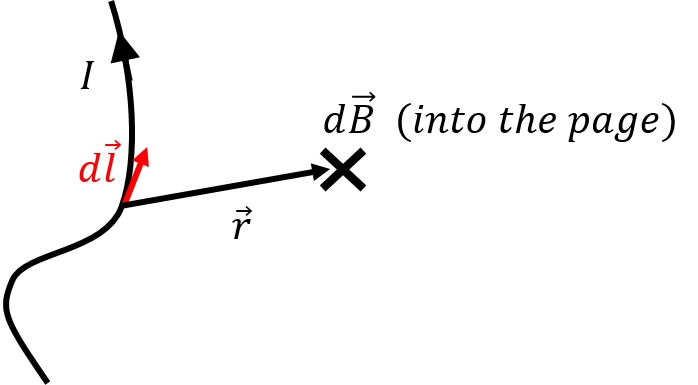
\includegraphics[width=0.5\linewidth]{files/biotsavart-37ffa7dec2527c7a20273b520610411d.png}
\caption[]{The infinitesimal magnetic field, $d\vec B$, that is created by an infinitesimal section of wire, $d\vec l$, carrying current $I$. Note that the vector, $\vec r$, goes from $d\vec l$ to the point where we wish to calculate the field.}
\label{fig:magneticsource:biotsavart}
\end{figure}

The Biot-Savart Law has some similarities with the Coulomb Law to calculate the electric field, as the magnitude of the magnetic field decreases as the inverse of the square distance between the source and the field. However, it can only be expressed in differential form (i.e. as an infinitesimal) and it requires working in three dimensions because of the cross product. It is usually more convenient to use the Biot-Savart Law in the form:
\begin{equation}
d\vec B = \frac{\mu_0 I}{4\pi}\frac{d\vec l\times \vec r}{r^3}
\end{equation}
where the unit vector $\hat r$ was replaced by $\vec r/r$.

The procedure for applying the Biot-Savart Law is as follows:

\begin{enumerate}
\item Make a really good diagram, as you will have to include some 3D aspects.
\item Choose an infinitesimal section of wire, $d\vec l$.
\item Determine the vector $\vec r$.
\item Determine the cross-product, $d\vec l \times \vec r$, which will point in the direction of the magnetic field from that infinitesimal section of wire.
\item Write out the infinitesimal vector $d\vec B$, and determine its components.
\item Think about symmetry! As you sum the $d\vec B$, will some components cancel? If yes, you do not need to do those integrals.
\item Determine the total magnetic field, component by component, by summing (integrating) the components of $d\vec B$ over the wire.
\end{enumerate}

\paragraph{Magnetic field from a straight current-carrying wire}

In this section, we use the Biot-Savart Law to determine the magnetic field a distance, $h$, from the centre of a finite straight wire of length $L$, carrying current $I$, as illustrated in Figure~\ref{fig:magneticsource:bswire}.

\begin{figure}[!htbp]
\centering
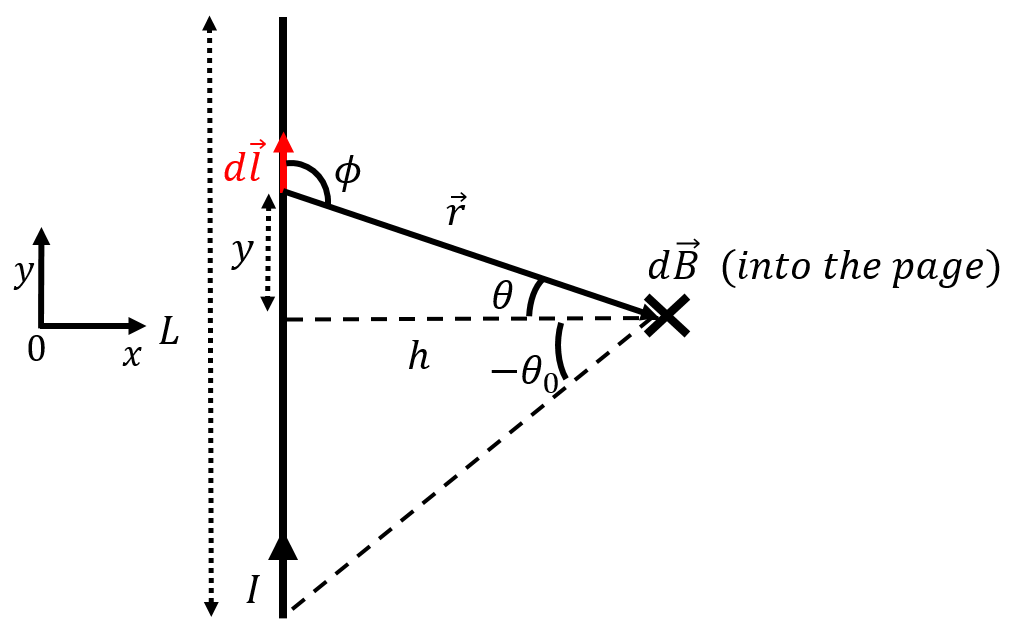
\includegraphics[width=0.7\linewidth]{files/bswire-dc40e864732d43d30aeb03f08e4a9a7e.png}
\caption[]{Setting up the model to use the Biot-Savart Law to calculate the magnetic field a distance $h$ from the centre of a current-carrying wire of length $L$.}
\label{fig:magneticsource:bswire}
\end{figure}

We start by choosing an infinitesimal element of wire, $d\vec l$, a distance $y$ above the centre of the wire, as shown (we choose the origin to be located at the centre of the wire). The vector $d\vec l$ is thus given by:
\begin{equation}
d\vec l = dl\hat y
\end{equation}
The vector, $\vec r$, from $d\vec l$ to the point at which we would like to know the magnetic field is given by:
\begin{equation}
\vec r &= r\cos\theta\hat x -r\sin\theta\hat y\\
r &=\sqrt{h^2+y^2} =\frac{h}{\cos\theta}
\end{equation}
The cross-product between $d\vec l$ and $\vec r$ is easily found with the right-hand rule to point into the page (corresponding to the negative $z$ direction). The magnitude of the cross-product is given by:
\begin{equation}
||d\vec l \times \vec r||=dl r \sin\phi
\end{equation}
where $\phi=\pi/2+\theta$ is the angle between $d\vec l$ and $\vec r$, so that $\sin\phi=\cos\theta$. The cross-product can thus be written in terms of $\theta$ as:
\begin{equation}
d\vec l \times \vec r=-dl r \cos\theta \hat z
\end{equation}
Note that we can also determine the cross-product algebraically instead of using the right-hand rule and the magnitude:
\begin{equation}
d\vec l \times \vec r &= (dl\hat y) \times (r\cos\theta\hat x -r\sin\theta\hat y)\\
&=dlr\cos\theta (\hat y \times\hat x) - rdl\sin\theta(\hat y \times \hat y)\\
&=-dlr\cos\theta \hat z
\end{equation}
The infinitesimal magnetic field element, $d\vec B$, is given by:
\begin{equation}
d\vec B = \frac{\mu_0 I}{4\pi}\frac{d\vec l\times \vec r}{r^3}=-\frac{\mu_0 I}{4\pi}\frac{dl\cos\theta}{r^2}\hat z
\end{equation}
Any segment along the wire will result in a magnetic field that is into the page (negative $z$ direction), thus there will be no cancellations due to any symmetries. We can now proceed to perform the integral.

We can use either $\theta$ or $y$ to label the wire elements and carry out the integration. We will choose to integrate over $\theta$, requiring us to express $dl$ and $r$ in terms of $\theta$ (and constants), as those are the only quantities in $d\vec B$ that depend on the position of $d\vec l$. In order to express $dl$ in terms of $d\theta$, we first relate $\theta$ to $y$, the position of the wire element:
\begin{equation}
y = h\tan\theta\quad \to \quad
dl = dy = \frac{dy}{d\theta}d\theta = \frac{h}{\cos^2\theta}d\theta
\end{equation}
and $r$ is given by:
\begin{equation}
r=\frac{h}{\cos\theta}\quad \to \quad
\frac{1}{r^2}&=\frac{\cos^2\theta}{h^2}
\end{equation}
Putting this altogether into $d\vec B$:
\begin{equation}
d\vec B &=-\frac{\mu_0 I}{4\pi}\frac{dl\cos\theta}{r^2}\hat z\\
&= -\frac{\mu_0 I}{4\pi}\left(\frac{h}{\cos^2\theta}d\theta\right) \left( \frac{\cos^2\theta}{h^2} \right)\cos\theta\hat z\\
&=-\frac{\mu_0 I}{4\pi h}\cos\theta d\theta \hat z=dB_z\hat z
\end{equation}
We define the angle, $\theta_0$, to be the maximum amplitude of the angle $\theta$ when integrating over the wire (see Figure~\ref{fig:magneticsource:bswire}), so that we integrate $\theta$ from $-\theta_0$ to $+\theta_0$:
\begin{equation}
B_z&=\int_{-\theta_0}^{+\theta_0}dB_z\\
&= -\frac{\mu_0 I}{4\pi h} \int_{-\theta_0}^{+\theta_0}\cos\theta d\theta\\
&=-\frac{\mu_0 I}{4\pi h}(2\sin\theta_0)\\
&=-\frac{\mu_0 I}{2\pi h}\sin\theta_0
\end{equation}
Using the given dimensions:
\begin{equation}
\sin\theta_0&=\frac{L/2}{\sqrt{h^2+\frac{L^2}{4}}}\\
\end{equation}
Thus, the magnetic field, $\vec B$, a distance, $h$, from the centre of a wire of length, $L$, carrying current, $I$, in the positive $y$ direction is given by:
\begin{equation}
\boxed{\vec B = -\frac{\mu_0 I}{2\pi h}\frac{L/2}{\sqrt{h^2+\frac{L^2}{4}}}\hat z}\quad\text{(finite wire)}
\end{equation}
The magnetic field must be rotationally symmetric; that is, if the wire is vertical, the magnetic field at a distance $h$ must look the same regardless of the angle from which we view the vertical wire (we should always see the magnetic field going into the page at the point that we use in Figure~\ref{fig:magneticsource:bswire}). Thus, the magnetic field lines must form circles around the wire, as illustrated in Figure~\ref{fig:magneticsource:wirefield}. Note that the direction of the magnetic field is given by the right-hand rule for axial vectors; when you align your thumb with the current, your fingers curl in the direction of the magnetic field.

\begin{figure}[!htbp]
\centering
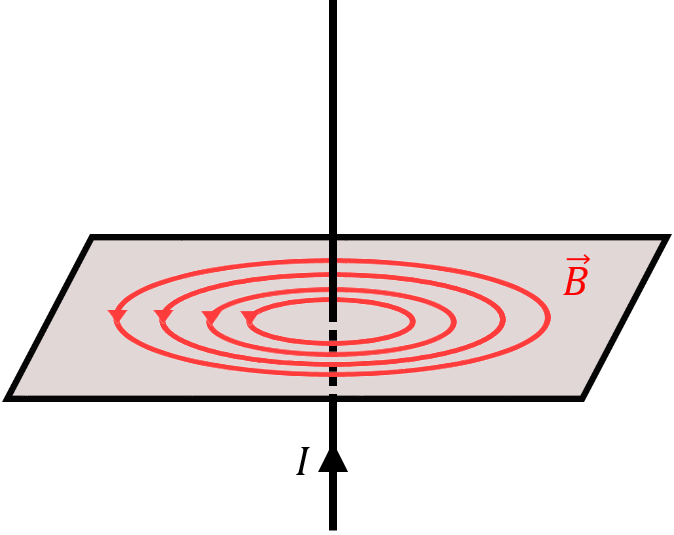
\includegraphics[width=0.4\linewidth]{files/wirefield-f0efa665a11f2b4ea619f8be5412e4f8.png}
\caption[]{The magnetic field from a current-carrying wire forms concentric circles centred on the wire.}
\label{fig:magneticsource:wirefield}
\end{figure}

It is of particular interest to investigate the limiting case of an infinitely long wire, in the limit of $L\to\infty$, or equivalently, $\theta_0\to\frac{\pi}{2}$. The latter is easiest to evaluate, since $\sin\theta_0\to 1$. The magnitude of the magnetic field, $\vec B$, a distance, $h$, from an infinite wire carrying current, $I$, is given by:
\begin{equation}
\boxed{ B = \frac{\mu_0 I}{2\pi h}}\quad\text{(infinite wire)}
\end{equation}
One can often make the approximation that the wire is infinite in length, when the distance, $h$, is small compared to the length, $L$, of the wire.

\paragraph{Magnetic field from a circular current-carrying wire}

In this section, we examine the magnetic field that is created by a circular current-carrying loop of wire. We can determine the shape of the magnetic field, by considering small sections as straight wires, with circular magnetic field lines around them. As we move closer to the centre of the ring, those fields sum together, as illustrated in Figure~\ref{fig:magneticsource:ringfield}. Note that the magnetic field from a loop of current is identical to that from a bar magnet (as a bar magnet is, of course, a collection of current loops).

\begin{figure}[!htbp]
\centering
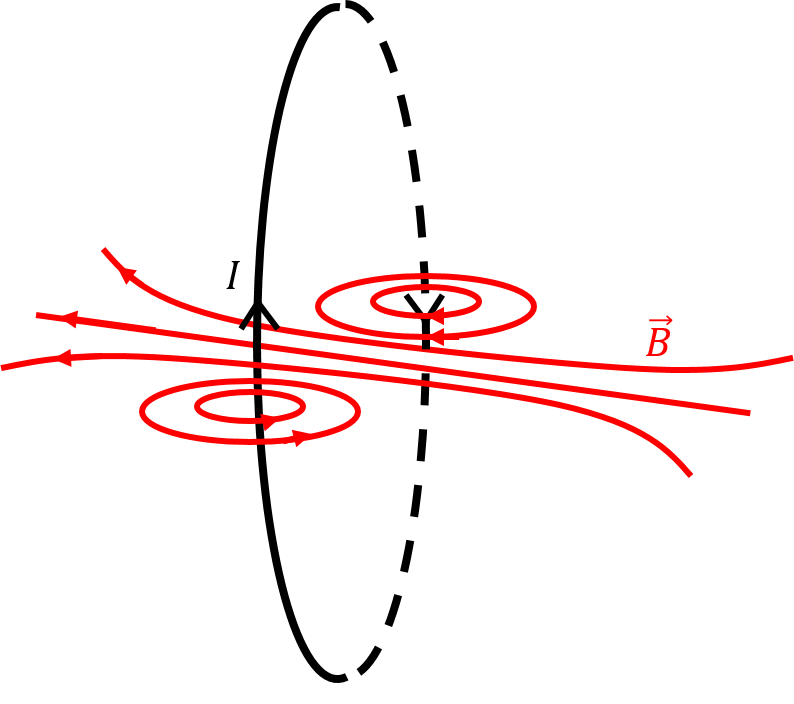
\includegraphics[width=0.4\linewidth]{files/ringfield-f13bccba775229de52496b9398a5ad25.png}
\caption[]{The magnetic field from a current-carrying loop of wire can be thought of as the sum of the fields from small straight sections of wire.}
\label{fig:magneticsource:ringfield}
\end{figure}

Below, we use the Biot-Savart Law to derive an expression for the magnitude of the magnetic field at a distance, $h$, from the centre of a ring of radius, $R$, along its axis of symmetry, when there is a current, $I$, in the ring. While the mathematics are much easier than the case for the straight wire, the challenge in this case is to visualize the calculation in three dimensions! Figure~\ref{fig:magneticsource:bsring} shows the loop of current, as well as our choice of coordinate system (with the origin at the centre of the ring). In particular, we wish to calculate the magnetic field at a distance, $h$, along the $z$ axis. The $x$ axis goes into the page.

\begin{figure}[!htbp]
\centering
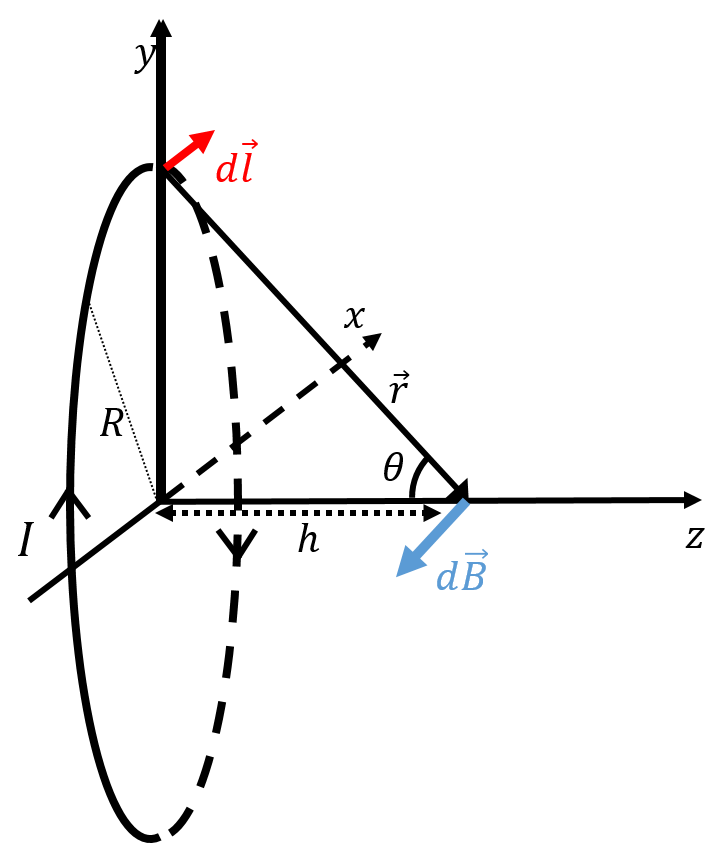
\includegraphics[width=0.4\linewidth]{files/bsring-740662e1ad7007d0abe905f8a7c59235.png}
\caption[]{Diagram to apply the Biot-Savart Law in order to determine the magnetic field along the symmetry axis of a ring carrying current, $I$. The $x$ axis goes into the page.}
\label{fig:magneticsource:bsring}
\end{figure}

In order to apply the Biot-Savart Law, we choose an element, $d\vec l$, of wire at the top of the ring, as illustrated. At this position, the element, $d\vec l$, points in the positive $x$ direction (into the page):
\begin{equation}
d\vec l = dl \hat x
\end{equation}
The vector, $\vec r$, from the wire element to the point where we wish to determine the magnetic field is given by:
\begin{equation}
\vec r =  - r\sin\theta \hat y+r\cos\theta \hat z
\end{equation}
and the angle $\theta$ will be the same for all wire elements along the ring. The cross-product, $d\vec l \times \vec r$, can be evaluated algebraically:
\begin{equation}
d\vec l \times \vec r &= (dl \hat x) \times ( - r\sin\theta \hat y+r\cos\theta \hat z)\\
&=-rdl\sin\theta (\hat x \times \hat y) + rdl\cos\theta (\hat x \times \hat z)\\
&=-rdl\sin\theta\hat z + rdl\cos\theta (-\hat y)\\
&=-rdl\sin\theta\hat z - rdl\cos\theta \hat y
\end{equation}
so that the element of magnetic field, $d\vec B$, corresponding to that choice of $d\vec l$, will lie in the $y -z$ plane, as illustrated in Figure~\ref{fig:magneticsource:bsring}. Note that the vector $d\vec B$ is perpendicular to the vector $\vec r$ (since it is the cross-product of $\vec r$ with another vector). The magnetic field element, $d\vec B$, is given by:
\begin{equation}
d\vec B &= \frac{\mu_0 I}{4\pi}\frac{d\vec l\times \vec r}{r^3}\\
&= \frac{\mu_0 I}{4\pi r^3}(-rdl\sin\theta\hat z - rdl\cos\theta \hat y )\\
&=\frac{\mu_0 I}{4\pi r^2}(-dl\sin\theta \hat z - dl\cos\theta \hat y)\\
&=dB_z\hat z + dB_y \hat y
\end{equation}
As the wire element, $d\vec l$, moves around the circle, the tip of the resulting magnetic field vector element traces a circle centred on the $z$ axis, as illustrated in Figure~\ref{fig:magneticsource:bsring_all}. Note that, in general, $d\vec B$ will also have an $x$ component (the $x$ component was only 0 before because we chose $d\vec l$ to be at the top of the ring). When we sum together the magnetic field elements, the $x$ and $y$ components will cancel, so that we are left with the $z$ component.

\begin{figure}[!htbp]
\centering
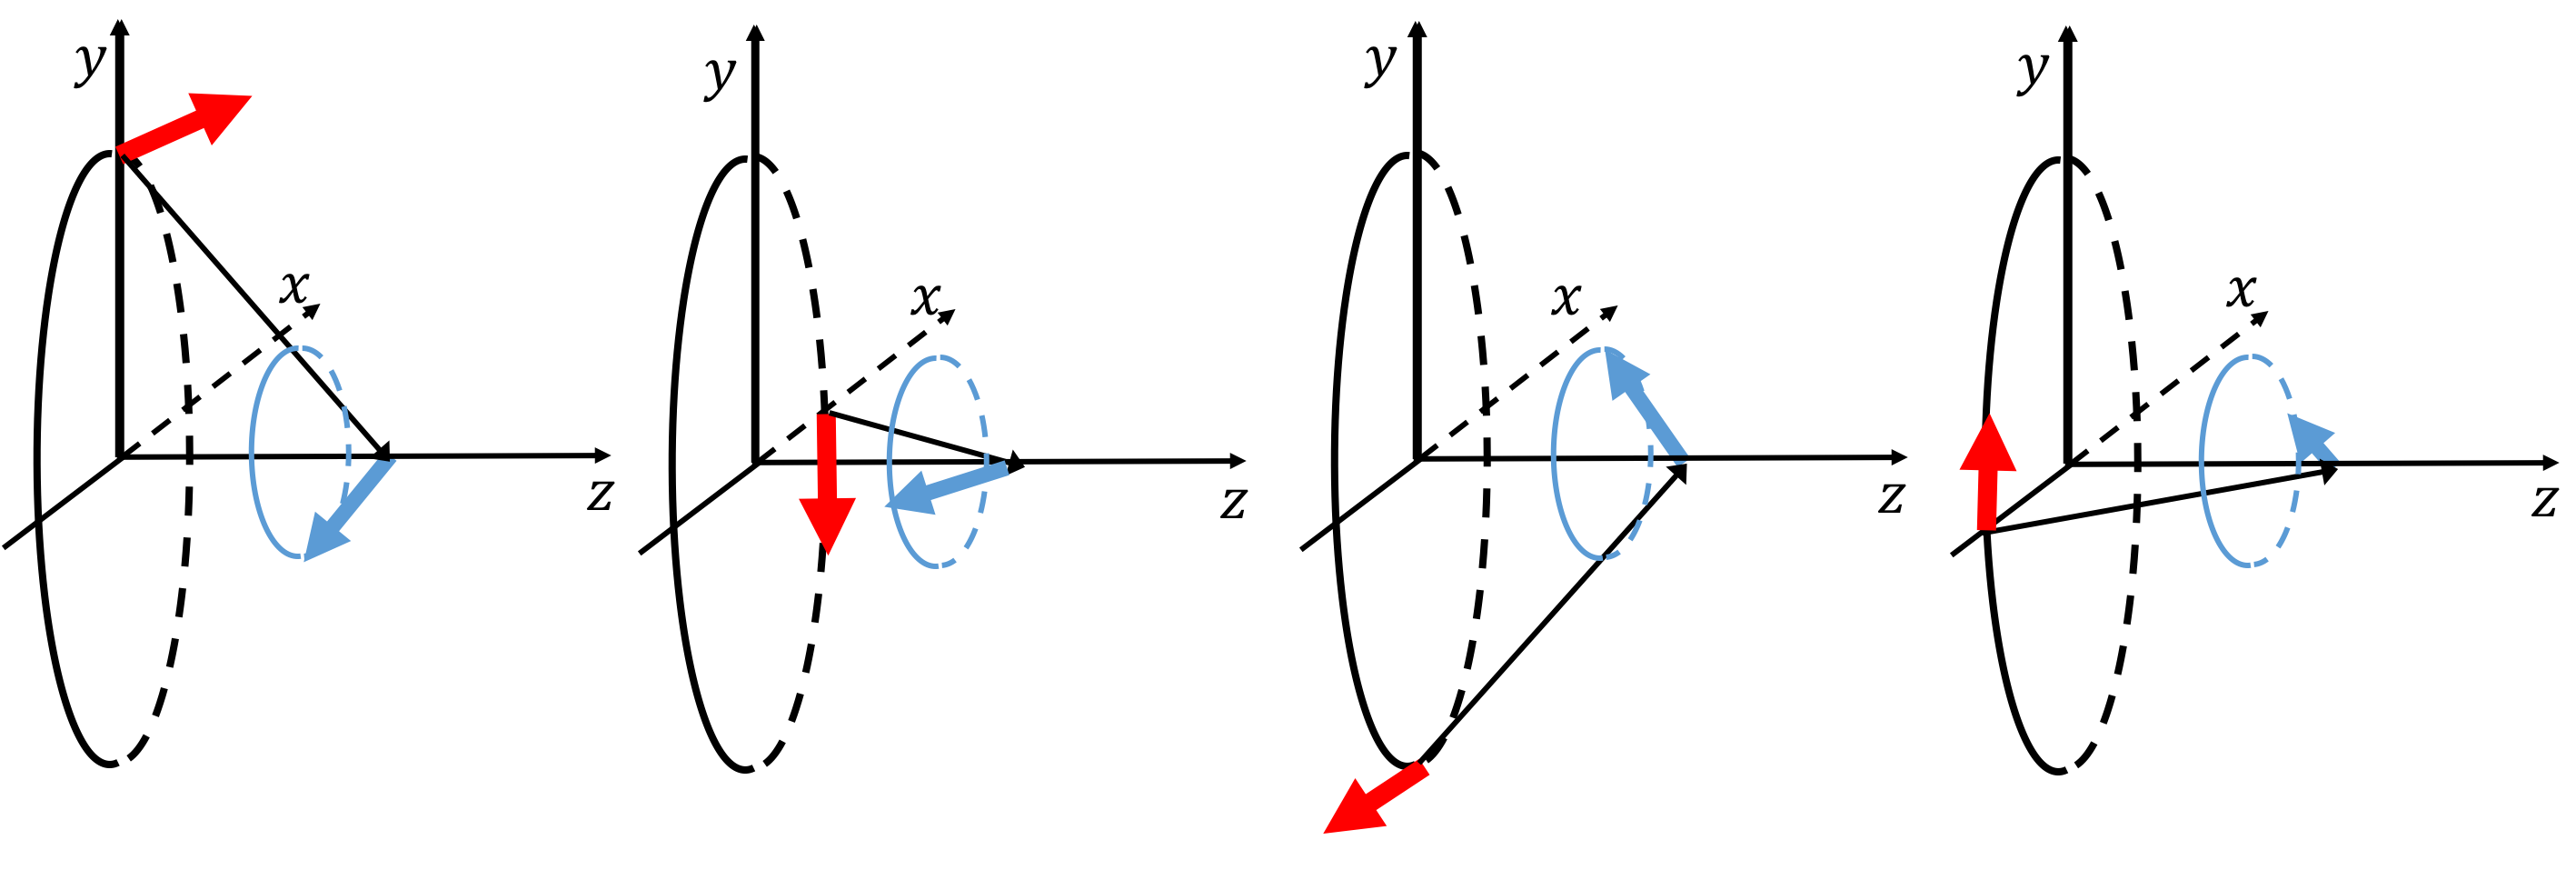
\includegraphics[width=0.9\linewidth]{files/bsring_all2-afdddcb12c4885a8783bea9825fd9214.png}
\caption[]{As the wire element, $d\vec l$, moves along the ring, the tip of corresponding magnetic field element vector, $d\vec B$, describes a circle centred on the $z$ axis. Thus, only the (negative) $z$ component of $d\vec B$ will survive when these are all added together.}
\label{fig:magneticsource:bsring_all}
\end{figure}

The total magnetic field will be in the negative $z$ direction, as anticipated from Figure~\ref{fig:magneticsource:ringfield}. Summing together the $z$ components of the infinitesimal magnetic fields:
\begin{equation}
dB_z &= -\frac{\mu_0 I}{4\pi r^2}dl\sin\theta\\
B_z &= \int dB_z\\
&=-\int \frac{\mu_0 I}{4\pi r^2}dl\sin\theta
\end{equation}
Note that in this case, both $r$ and $\theta$ are constant for all of the $d\vec l$, allowing us to take them out of the integral. The integral is then just a sum of the $dl$ elements, which must add up to the circumference of the ring:
\begin{equation}
B_z &= \int dB_z\\
&= -\frac{\mu_0 I}{4\pi r^2}\sin\theta \int_0^{2\pi R} dl\\
&=-\frac{\mu_0 I}{4\pi r^2}\sin\theta (2\pi R)\\
&=-\frac{\mu_0 I}{2r^2}R\sin\theta
\end{equation}
In terms of the variables that we are given:
\begin{equation}
r &= \sqrt{R^2+h^2}\\
\sin\theta &=\frac{R}{r}=\frac{R}{\sqrt{R^2+h^2}}\\
\end{equation}
\begin{equation}
\therefore\;\; \boxed{\vec B = -\frac{\mu_0 I}{2} \frac{R^2}{(R^2+h^2)^\frac{3}{2}} \hat z}\quad\text{(field from a loop of current)}
\end{equation}
In this case, the math was relatively straightforward (no substitutions to evaluate the integral), however it is challenging to visualize the problem in three dimensions.

\begin{framed}
\textbf{Checkpoint}\\
A coil is made of $N$ loops of current-carrying wire packed closely together. What is the magnetic field at the centre of the coil?

\begin{enumerate}
\item $\frac{\mu_0I}{2R}$
\item $\frac{N\mu_0I}{2R}$
\item $\frac{N\mu_0I}{2R^2}$
\item $\frac{\mu_0I}{R}$
\end{enumerate}

\begin{framed}
\textbf{Answer}\\
\begin{enumerate}[resume]
\item
\end{enumerate}
\end{framed}
\end{framed}

\subsubsection{Force between two current-carrying wires}

Consider two infinite parallel straight wires, a distance $h$ apart, carrying upwards currents, $I_1$ and $I_2$, respectively, as illustrated in Figure~\ref{fig:magneticsource:twowires}.

\begin{figure}[!htbp]
\centering
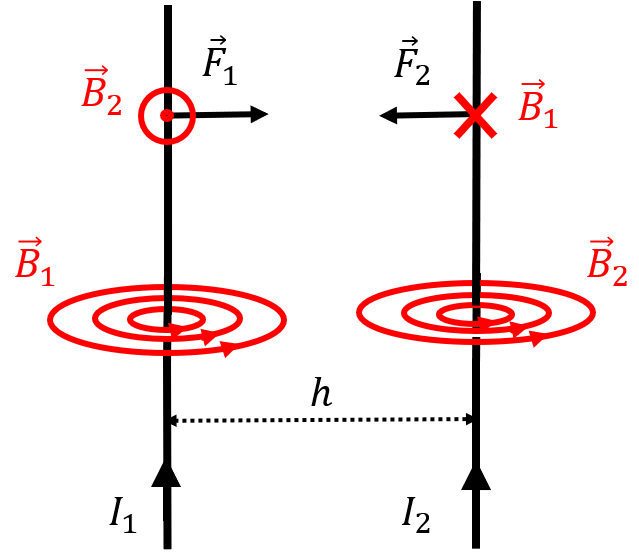
\includegraphics[width=0.4\linewidth]{files/twowires-c728efaf080baf12aff491b194a58f14.png}
\caption[]{Two parallel current-carrying wires will exert an attractive force on each other, if their currents are in the same direction.}
\label{fig:magneticsource:twowires}
\end{figure}

The first wire will create a magnetic field, $\vec B_1$, in the shape of circles concentric with the wire. At the position of the second wire, the magnetic field $B_1$ is into the page, and has a magnitude:
\begin{equation}
B_1 = \frac{\mu_0 I_1}{2\pi h}
\end{equation}
Since the second wire carries a current, $I_2$, upwards, it will experience a magnetic force, $\vec F_2$, from the magnetic field, $B_1$, that is towards the left (as illustrated in Figure~\ref{fig:magneticsource:twowires} and determined from the right-hand rule). The magnetic force, $\vec F_2$, exerted on a section of length, $l$, on the second wire has a magnitude given by:
\begin{equation}
F_2 = I_2 ||\vec l \times \vec B_1||=I_2 l B_1 =\frac{\mu_0 I_2 I_1 l}{2\pi h}
\end{equation}
where we used the fact that the angle between $\vec l$ and $\vec B$ is $90 {\rm \degree}$. We expect, from Newton's Third Law, that an equal and opposite force should be exerted on the first wire. Indeed, the second wire will create a magnetic field, $\vec B_2$, that is out of the page at the location of the first wire, with magnitude:
\begin{equation}
B_2 = \frac{\mu_0 I_2}{2\pi h}
\end{equation}
This leads to a magnetic force, $\vec F_1$, exerted on the first wire, that points to the right (from the right-hand rule). On a section of length, $l$, of the first wire, the magnetic force from the magnetic field, $\vec B_2$, has magnitude:
\begin{equation}
F_1 = I_1 ||\vec l \times \vec B_2||=I_1 l B_2 =\frac{\mu_0 I_1 I_2}{2\pi h}
\end{equation}
which does indeed have the same magnitude as the force exerted on the second wire. Thus, when two parallel wires carry current in the same direction, they exert equal and opposite attractive forces on each other.

\begin{framed}
\textbf{Checkpoint}\\
\begin{figure}[!htbp]
\centering
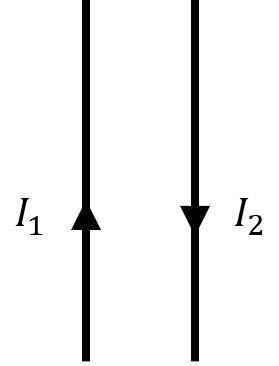
\includegraphics[width=0.2\linewidth]{files/oppositewires-db434c55df786bbeaad218aa318228be.png}
\caption[]{Two wires that carry current in opposite directions.}
\label{fig:magneticsource:oppositewires}
\end{figure}

Two parallel wires carry current in opposite directions, as shown in Figure~\ref{fig:magneticsource:oppositewires}. What force do they exert on each other?

\begin{enumerate}
\item There will be no force, since the currents cancel.
\item There will be an attractive force between the wires.
\item There will be a repulsive force between the wires.
\end{enumerate}

\begin{framed}
\textbf{Answer}\\
\begin{enumerate}[resume]
\item
\end{enumerate}
\end{framed}
\end{framed}

The attractive force between two wires used to be the basis for defining the Ampère, the S.I. (base) unit for electric current. Before 2019, the Ampère was defined to be ``that constant current which, if maintained in two straight parallel conductors of infinite length, of negligible circular cross-section, and placed one metre apart in vacuum, would produce between these conductors a force equal to $2\times 10^{ -17} {\rm N}$ per metre of length''. Recently, the definition was updated to be based on defining the Coulomb in such a way that the elementary charge has a numerical value of $e=1.602176634\times 10^{ -19} {\rm C}$, and the Ampère corresponds to one Coulomb per second.

The force between two wires is a good system to understand how any physical quantity cannot depend on our choice of the right-hand to define cross-products. As mentioned in the previous chapter, any physical quantity, such as the direction of the force exerted on a wire, will always depend on two successive uses of the right hand. In this system, we first used the right-hand rule for axial vectors to determine the direction of the magnetic field from one of the wires. We then used the right-hand rule to determine the direction of the cross-product to determine the direction of the force on the other wire. You can verify that you get the same answer if you, instead, use your left-hand to define the direction of the magnetic field (which will be in the opposite direction), and then again for the cross-product. This also highlights that the magnetic field (and the electric field) is just a mathematical tool that we use to, ultimately, describe the motion of charges or compass needles.

\begin{framed}
\textbf{Olivia's Thoughts}\\
For this problem, we can determine whether the force is attractive or repulsive by finding the directions of  the forces on wire 1 ($\vec{F_1}$) and wire 2 ($\vec{F_2}$). Figure~\ref{fig:magneticsource:2wires_steps} shows how to find the directions of $\vec{F_1}$ and $\vec{F_2}$ step by step using the right hand rules. The process is as follows:

\begin{enumerate}
\item Use the axial right hand rule to find the magnetic field at wire 2 due to the current in wire 1 ($\vec{B_1}$).
\item Use the right hand rule to find the direction of the force on wire 2 due to its current and the magnetic field $\vec{B_1}$.
\item Use the axial right hand rule to find the magnetic field at wire 1 due to the current in wire 2 ($\vec{B_2}$).
\item Use the right hand rule to find the direction of the force on wire 1 due to its current and the magnetic field $\vec{B_2}$.
\end{enumerate}

\begin{figure}[!htbp]
\centering
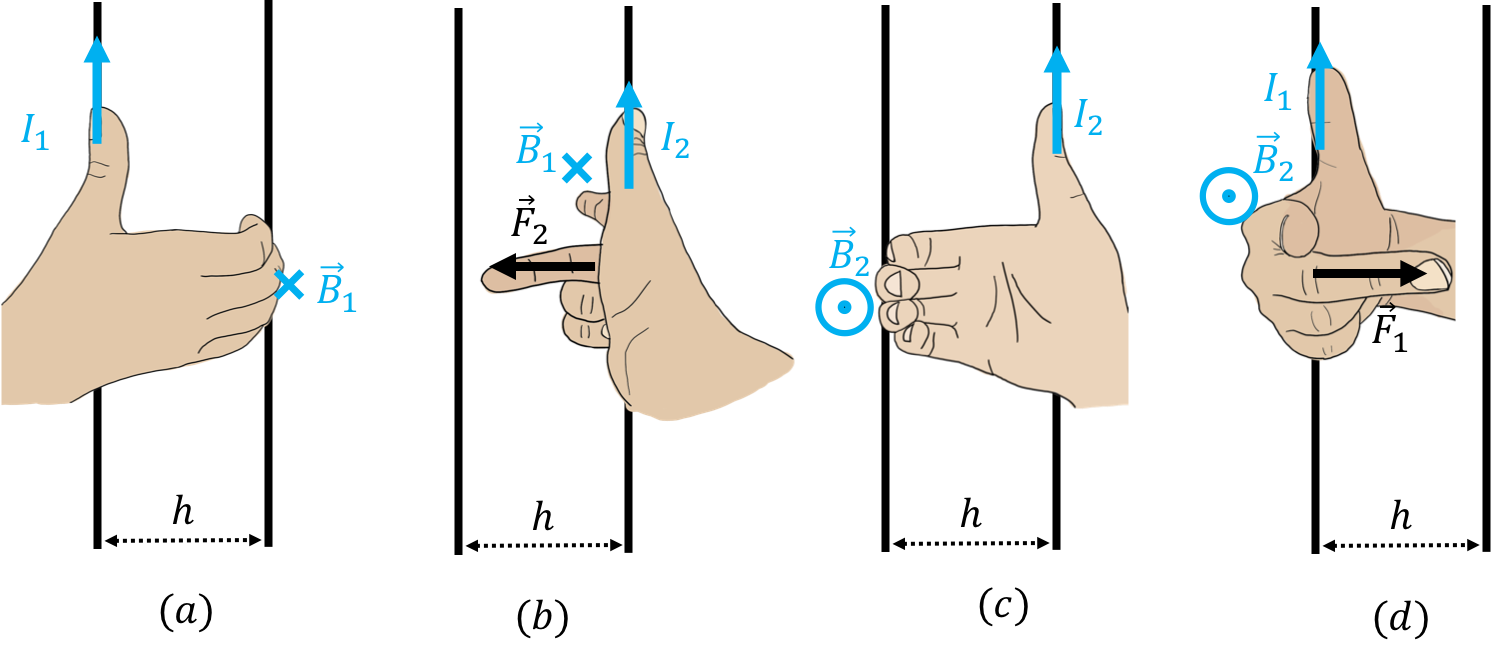
\includegraphics[width=0.8\linewidth]{files/2wire_rhr-c435f687470e9436439dd1962c8d6354.png}
\caption[]{(a) Axial right hand rule to find $\vec{B_1}$. (b) Right hand rule to find $\vec{F_2}$. (c) Axial right hand rule to find $\vec{B_2}$. (d) Right hand rule to find $\vec{F_1}$.}
\label{fig:magneticsource:2wires_steps}
\end{figure}

Both $\vec{F_1}$ and $\vec{F_2}$ point towards the centre, so the force is attractive. See what happens when you use your left hand!
\end{framed}

\begin{framed}
\textbf{Checkpoint}\\
When current is flowing in a straight cable, how to you expect the charges to be distributed radially through the cross-section of the cable?

\begin{enumerate}
\item Uniformly in radius (current density does not depend on $r$).
\item There will be an excess of positive charges on the outside of the cable.
\item There will be an excess of negative charges on the outside of the cable.
\end{enumerate}

\begin{framed}
\textbf{Answer}\\
\begin{enumerate}[resume]
\item
\end{enumerate}
\end{framed}
\end{framed}

\subsubsection{Ampère's Law}

Ampère's Law is similar to Gauss' Law, as it allows us to (analytically) determine the magnetic field that is produced by an electric current in configurations that have a high degree of symmetry. Ampère's Law states:
\begin{equation}
\boxed{\oint \vec B \cdot d\vec l =\mu_0 I^{enc}}
\end{equation}
where the integral on the left is a ``path integral'', similar to how we calculate the work done by a force over a particular path. The circle sign on the integral means that this is an integral over a ``closed'' path; a path where the starting and ending points are the same. $I^{enc}$ is the net current that crosses the surface that is defined by the closed path, often called the ``current enclosed'' by the path. This is different from Gauss' Law, where the integral is over a closed surface (not a closed path, as it is here). In the context of Gauss' Law, we refer to ``calculating the \textbf{flux} of the electric field \textbf{through} a closed surface''; in the context of Ampère's Law, we refer to ``calculating the \textbf{circulation} of the magnetic field \textbf{along} a closed path''.

We apply Ampère's Law in much the same way as we apply Gauss' Law:

\begin{enumerate}
\item Make a good diagram, identify symmetries.
\item Choose a closed path over which to calculate the circulation of the magnetic field (see below for how to choose the path). The path is often called an ``Amperian loop'' (think ``Gaussian surface'').
\item Evaluate the circulation integral.
\item Determine how much current is ``enclosed'' by the Amperian loop.
\item Apply Ampère's Law.
\end{enumerate}

Similarly to Gauss' Law, we need to \textbf{choose the path} (instead of the surface) over which we will evaluate the integral. The integral will be easy to evaluate if:

\begin{enumerate}
\item \textbf{The angle between $\vec B$ and $d\vec l$ is constant along the path}, so that:
\end{enumerate}
\begin{equation}
\oint  \vec B \cdot d\vec l = \oint B dl \cos\theta = \cos\theta \oint B dl
\end{equation}
where $\theta$ is the angle between $\vec B$ and $d\vec l$.

\begin{enumerate}[resume]
\item \textbf{The magnitude of $\vec B$ is constant along the path}, so that:
\end{enumerate}
\begin{equation}
\cos\theta \oint B dl = B\cos\theta \oint dl
\end{equation}
Choosing a path that meets these two conditions is only possible if there is a high degree of symmetry.

Consider an infinitely long straight wire, carrying current, $I$, out of the page, as illustrated in Figure~\ref{fig:magneticsource:amperewire}. The magnetic field from the wire must look the same regardless of the angle from which we view the wire (``azimuthal symmetry''). Thus, the magnetic field must either form concentric circles around the wire (which we know is the case from the Biot-Savart Law) or it must be in the radial direction (pointing towards or away from the wire). These two possibilities are illustrated in Figure~\ref{fig:magneticsource:amperewire}, and we will pretend, for now, that we do not know which is correct.

\begin{figure}[!htbp]
\centering
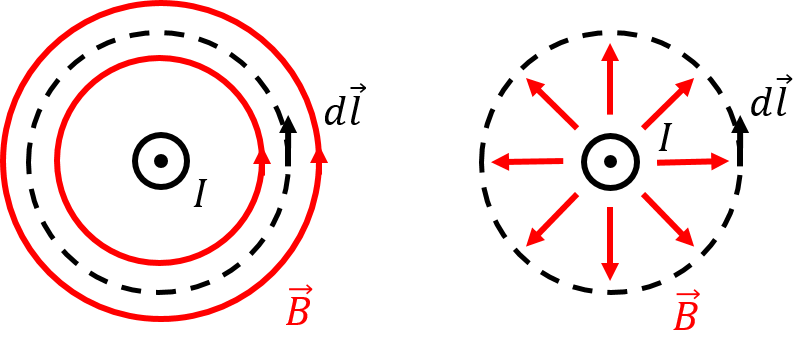
\includegraphics[width=0.6\linewidth]{files/amperewire-472189ba3763707d7ea318766a8855fb.png}
\caption[]{By symmetry, the magnetic field from a current-carrying infinite wire (illustrated with current coming out of the page), must either form concentric circles (left panel), or be in the radial direction (right panel). We know that the former (circles, left panel) is the correct choice. The dotted lines show ``Ampèrian loops'' that one can use to calculate the integral in Ampère's Law.}
\label{fig:magneticsource:amperewire}
\end{figure}

In order to apply Ampère's Law, we choose an Amperian loop (instead of a ``Gaussian surface''). In the case of an infinite current-carrying wire, a circle that is concentric with the wire will meet the properties above, regardless of the two possible configurations of the magnetic field: with a circular Amperian loop, the angle between the magnetic field and the element $d\vec l$ is constant along the entire loop, and the magnitude of the magnetic field is constant along the loop. Our choice of loop is illustrated in Figure~\ref{fig:magneticsource:amperewireloop}, where we have illustrated the magnetic field for the case where it forms concentric circles.

\begin{figure}[!htbp]
\centering
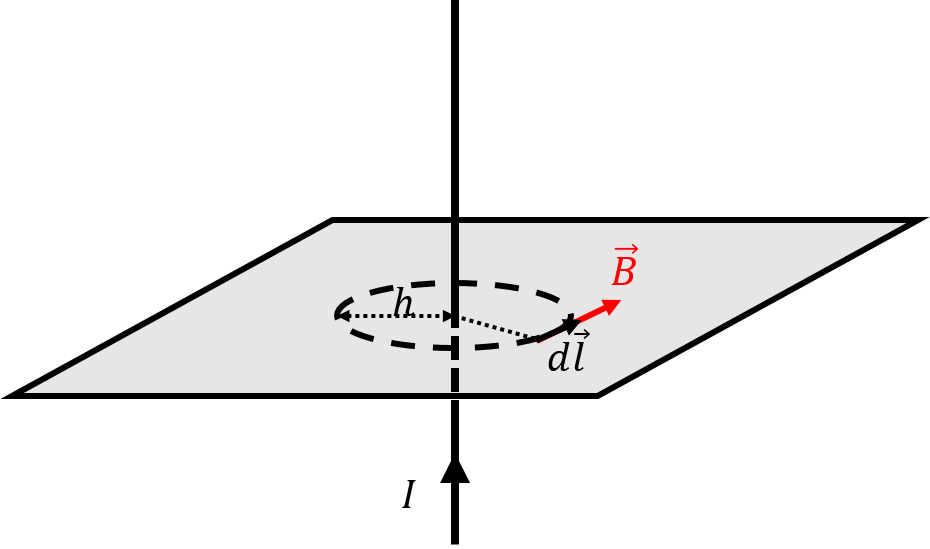
\includegraphics[width=0.5\linewidth]{files/amperewireloop-b47f54367ef17bf0efcd9e449152a81b.png}
\caption[]{An Amperian loop that is a circle of radius, $h$, will allow us to determine the magnetic field at a distance, $h$, from an infinitely-long current-carrying wire.}
\label{fig:magneticsource:amperewireloop}
\end{figure}

The circulation of the magnetic field along a circular path of radius, $h$, is given by:
\begin{equation}
\oint  \vec B \cdot d\vec l = \oint B dl \cos\theta = \cos\theta \oint B dl=B\cos\theta \oint dl=B\cos\theta (2\pi h)
\end{equation}
where $\cos\theta$ is 1 if the field forms circles (correct) or 0 if the field is radial (incorrect). We can now evaluate the current that is enclosed by the Amperian loop. The current that is enclosed is given by the net current that traverses the surface defined by the Amperian loop (in this case, a circle of radius $h$). Since the loop encloses the entire wire, the enclosed current is simply $I$. Applying Ampère's Law:
\begin{equation}
\oint \vec B \cdot d\vec l &=\mu_0 I^{enc}\\
B\cos\theta (2\pi h) &= \mu_0 I
\end{equation}
At this point, it is clear that $\cos\theta$ cannot be zero, since the right-hand side of the equation is not zero. We can thus conclude that the magnetic field must indeed make concentric circles, as we had previously determined. The magnitude of the magnetic field is given by:
\begin{equation}
B = \frac{\mu_0 I}{2\pi h}
\end{equation}
as we found previously with the Biot-Savart Law. Again, in analogy with Gauss' Law, one needs to apply some knowledge of symmetry and argue in which direction the magnetic field should point, in order to use Ampère's Law effectively.

\begin{framed}
\textbf{Checkpoint}\\
Ampère's law proves that the magnetic field at the centre of a current-carrying loop is zero because there is no enclosed current:

\begin{enumerate}
\item True.
\item False.
\end{enumerate}

\begin{framed}
\textbf{Answer}\\
\begin{enumerate}[resume]
\item
\end{enumerate}
\end{framed}
\end{framed}

\begin{framed}
\textbf{Olivia's Thoughts}\\
Let's compare Ampere's law to Gauss's law. Recall that Gauss's law is given by:
\begin{equation}
\oint \vec{E}\cdot d\vec{A}=\frac{Q^{enc}}{\epsilon_0}.
\end{equation}
We want to construct a Gaussian surface such that we can write this as
\begin{equation}
EA=\frac{Q^{enc}}{\epsilon_0},
\end{equation}
where $A$ is the surface area that is perpendicular to the field lines and $E$ is the (constant) magnitude of the electric field over the surface. The flux is given by $Q^{enc}/\epsilon_0$. To find the electric field at any point on the surface, we use
\begin{equation}
E=\frac{Q^{enc}/\epsilon_0}{A}.
\end{equation}
In other words, the electric field is the flux per unit area. Ampère's law is very similar, except that instead of flux, we have the new concept of ``circulation'' and instead of a surface integral, we have a line integral. When we have a high degree of symmetry in Ampère's law, we are often able to write:
\begin{equation}
\oint \vec{B}\cdot d\vec{l}=\mu_0 I^{enc}\rightarrow Bl=\mu_0 I^{enc}
\end{equation}
where $l$ is the length of the Amperian loop that is parallel to the field, $B$ is the magnitude of the magnetic field, and $\mu_0 I^{enc}$ gives us the circulation. To find the magnetic field, we use
\begin{equation}
B=\frac{\mu_0 I^{enc}}{l},
\end{equation}
so the magnetic field is like the circulation per unit length.

In the left panel of Figure~\ref{fig:magneticsource:amperecirculation}, I have shown two Amperian loops with different radii, for the example of the straight wire with a current coming out of the page. Ampère's law tells us that the circulation will be the same along each path. However, because the inner loop is smaller, the circulation per unit length (the magnetic field) will be larger at each point. This is represented in the right panel, where the length of the vectors is proportional to the magnetic field strength.

\begin{figure}[!htbp]
\centering
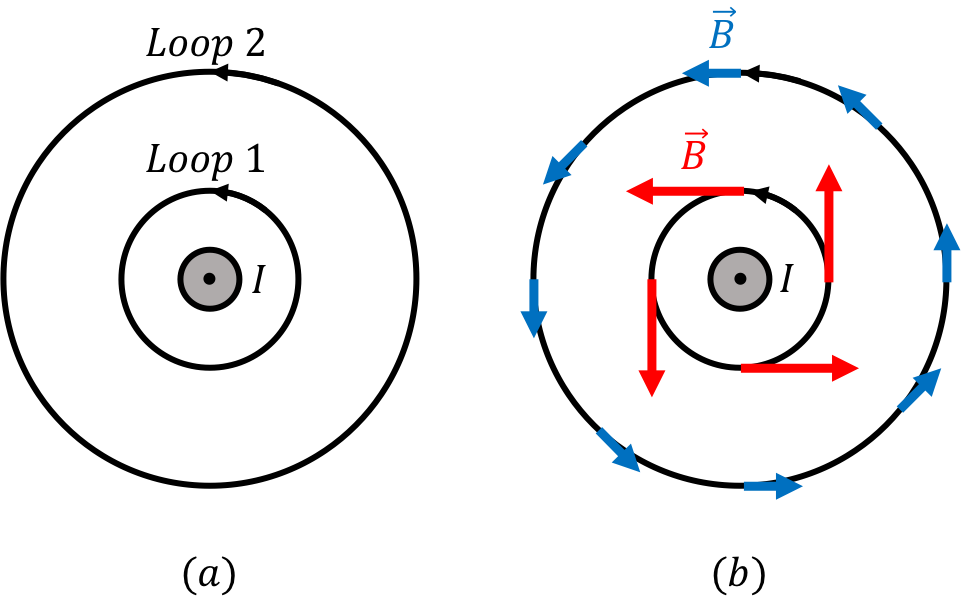
\includegraphics[width=0.6\linewidth]{files/Ampere_circulation-e38a2746744c28a733119cb646d86f03.png}
\caption[]{Left: 2 Amperian loops around a current carrying wire. Right: Magnetic field vectors around each loop.}
\label{fig:magneticsource:amperecirculation}
\end{figure}
\end{framed}

\begin{framed}
\textbf{Example 21.1}\\
A long solid uniform cable of radius, $R$, carries current, $I$, with a current density that is uniform through the cross-section of the cable. Determine the strength of the magnetic field as a function of $r$, the distance from the centre of the cable, inside \textit{and} outside of the cable.

\begin{framed}
\textbf{Solution}\\
In this case, we need to determine the magnetic field both inside and outside of the cable. Figure~\ref{fig:magneticsource:amperecable} shows two circular Amperian loops that we can use to apply Ampère's Law to determine the magnetic field inside and outside of the cable.

\begin{figure}[!htbp]
\centering
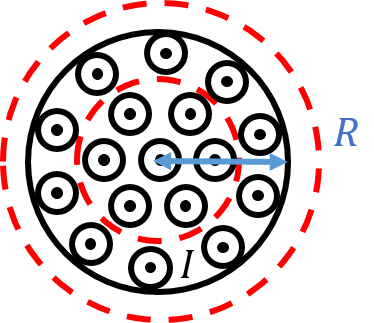
\includegraphics[width=0.4\linewidth]{files/amperecable-c842bce99807fda38aa74536705a03e7.png}
\caption[]{Two circular Amperian loops to determine the magnitude of the magnetic field inside and outside of a current-carrying cable of radius, $R$ (with uniform current coming out of the page).}
\label{fig:magneticsource:amperecable}
\end{figure}

By symmetry, and following the discussion in this chapter, we know that the magnetic field must form concentric circles, both inside and outside of the cable. Outside the cable, we proceed in the same fashion as above, choosing an Amperian loop of radius, $r>R$, such that the circulation is given by:
\begin{equation}
\oint \vec B \cdot d\vec l= B 2\pi r
\end{equation}
The entire cable is enclosed by the loop, so that the enclosed current is, $I$. Thus, Ampère's Law gives:
\begin{equation}
\oint \vec B \cdot d\vec l &=\mu_0 I^{enc}\\
B (2\pi r) &= \mu_0 I\\
\therefore B &= \frac{\mu_0 I}{2\pi r}\quad(r\geq R)
\end{equation}
Inside of the cable, the circulation integral around a circular path of radius, $r<R$, is the same:
\begin{equation}
\oint \vec B \cdot d\vec l= B 2\pi r
\end{equation}
However, in this case, the smaller Amperian loop does not enclose all of the current flowing through the cable. We are told that the current density, $j$, is uniform in the cable. We can thus determine the current per unit area (i.e. the current density) that flows through the whole cable, and use that to determine how much current flows through the surface with area $\pi r^2$ that is defined by the Amperian loop:
\begin{equation}
j &= \frac{I}{A}=\frac{I}{\pi R^2}\\
\therefore I^{enc} &= j(\pi r^2) = \frac{I}{\pi R^2}(\pi r^2)=I\frac{r^2}{R^2}
\end{equation}
Finally, we can apply Ampère's Law to determine the magnitude of the magnetic field inside the cable:
\begin{equation}
\oint \vec B \cdot d\vec l &=\mu_0 I^{enc}\\
B (2\pi r) &= \mu_0 I\frac{r^2}{R^2}\\
\therefore B &= \frac{\mu_0 I}{2\pi R^2}r
\end{equation}
and we find that the magnetic field is zero at the centre of the cable ($r=0$), and increases linearly up to the edge of the cable ($r=R$).

\textbf{Discussion:} In this example, we used Ampère's Law to model the strength of the magnetic field inside and outside of a current-carrying cable. In order to apply Ampère's Law inside the cable, we took into account that only a fraction of the current is enclosed by the Amperian loop. This problem is analogous to applying Gauss' Law to determine the electric field inside and outside of a uniformly charged sphere.
\end{framed}
\end{framed}

\paragraph{Interpretation of Ampère's Law and vector calculus}\label{sec:magneticsource:interpretation}

In this section, we discuss Ampère's Law in the context of vector calculus and provide a different perspective, mostly for informational purposes. The integral that appears in Ampère's Law is called the ``circulation'' of the vector field, $\vec B$:
\begin{equation}
\oint \vec B \cdot d\vec l
\end{equation}
The circulation, as its name implies, is a measure of ``how much rotation there is in the field''. To visualize this, imagine that the vector field is a velocity field for points in a fluid. Regions of the fluid where there are little whirlpools (so called ``eddies''), correspond to regions of the field with non-zero circulation (the sign of the integral tells us the direction of rotation, using the right-hand rule for axial vectors). Examples of field with and without circulation are shown in Figure~\ref{fig:magneticsource:circulation}. You will recognize that static electric charges create electric fields with no circulation (right panel), whereas static currents create magnetic fields with circulation.

\begin{figure}[!htbp]
\centering
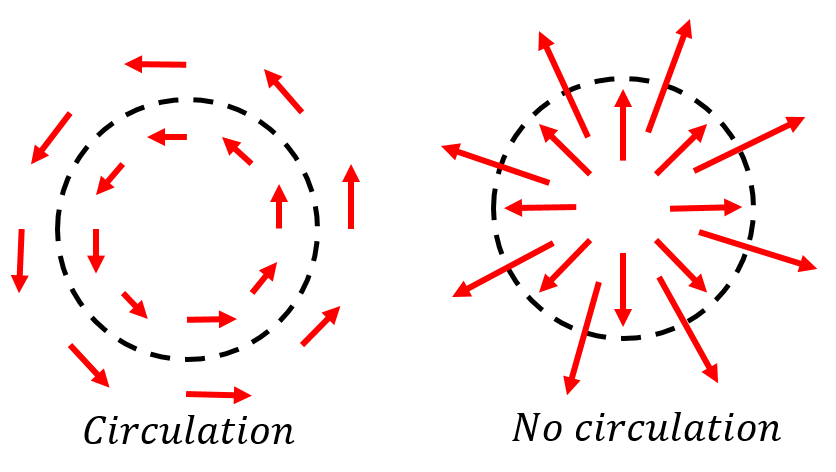
\includegraphics[width=0.5\linewidth]{files/circulation-e4d7d465e28a0d993fee414e2645c2bf.png}
\caption[]{Examples of field with (left panel) and without (right panel) circulation, as evaluated along the closed loop shown with the dashed line.}
\label{fig:magneticsource:circulation}
\end{figure}

Ampère's Law is thus a statement that an electric current will result in a field with a magnitude proportional to the current, that has some degree of rotation to it. The direction of rotation of that field corresponds to the right-hand rule for axial vectors as applied to the current (your thumb points in the direction of the current so that your fingers curl in the direction of the rotation of the associated field).

Circulation, as defined by the integral over a closed loop, is not a local property of the field, since it depends on what the field is doing as a whole over the path of the loop. Just as one can obtain a ``local'' version of  Gauss' Law, one can also obtain a local version of Ampère's Law using techniques from advanced vector calculus (that are beyond the scope of this textbook).

Stokes' theorem allows one to convert the circulation integral (a path integral on a closed loop) into a integral over the (open) surface that is defined by the loop:
\begin{equation}
\oint_C \vec B \cdot d\vec l = \int_S (\nabla \times \vec B) \cdot d\vec A
\end{equation}
where the subscript $C$ indicates that the integral is over a one-dimensional path, whereas the subscript $S$ indicates that the integral is over a two-dimensional surface. The term, $\nabla \times \vec B$, is called the ``curl'' of the magnetic field and is a local measure of the amount of rotation in the field. Applying Stokes' theorem to Ampère's Law yield:
\begin{equation}
\oint \vec B \cdot d\vec l &= \mu_0 I^{enc}\\
\int_S (\nabla \times \vec B) \cdot d\vec A &= \mu_0 I^{enc}\\
\end{equation}
Note that we can also write the current, $I^{enc}$, that is enclosed by the loop as the integral of the current density, $\vec j$, over the surface defined by the loop:
\begin{equation}
I^{enc}=\int _S \vec j \cdot d\vec A
\end{equation}
Thus, we can write Ampère's Law with integrals over the same surface on either side of the equation, implying that the integrands must be the same:
\begin{equation}
\int_S (\nabla \times \vec B) \cdot d\vec A = \mu_0 \int _S \vec j \cdot d\vec A\\
\end{equation}
\begin{equation}
\therefore\;\;\boxed{ \nabla \times \vec B = \mu_0 \vec j}
\end{equation}
This last equation now relates a local property (current density) to the magnetic field at that point, and is the usual form in which Ampère's Law is presented (the so-called ``differential form'', rather than the ``integral form'').

The curl of the magnetic field, $\nabla \times \vec B$, is a vector that is given by the following:
\begin{equation}
\nabla \times \vec B = \left(\frac{\partial B_z}{\partial y}-\frac{\partial B_y}{\partial z}\right)\hat x + \left(\frac{\partial B_x}{\partial z}-\frac{\partial B_z}{\partial x}\right)\hat y+\left(\frac{\partial B_y}{\partial x}-\frac{\partial B_x}{\partial y}\right)\hat z
\end{equation}
and the name ``curl'' is chosen because this is a measure of the amount of rotation (curl) in the field. In differential form, Ampère's Law can read as: ``a current density will create a (magnetic) field that has non-zero curl''.

Since Ampère's Law in differential form is a vector equation (both sides are vectors), it really corresponds to three equations in Cartesian coordinates, one per component. For example, the $x$ component of the equation is a ``partial differential equation'' for the $y$ and $z$ components of the magnetic field:
\begin{equation}
\left(\frac{\partial B_z}{\partial y}-\frac{\partial B_y}{\partial z}\right) &=\mu_0j_x
\end{equation}
that is in general difficult to solve without a computer (and all three equations are required, as these are ``coupled'', since a given component of the magnetic field appears in two of three equations).

\subsubsection{Solenoids and toroids}

In order to create strong magnetic fields, the most practical method is to combine many loops of current together into a ``solenoid'' (a coil). Electromagnets function on this principle and are ubiquitous in our lives. Figure~\ref{fig:magneticsource:solenoid1} shows the magnetic field from a single loop of current.

\begin{figure}[!htbp]
\centering
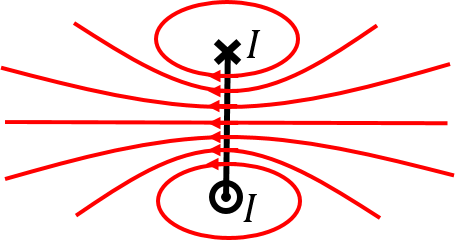
\includegraphics[width=0.3\linewidth]{files/solenoid1-ed94cf3c9ed3767449e82b299f74ebb5.png}
\caption[]{The magnetic field from a single loop of current.}
\label{fig:magneticsource:solenoid1}
\end{figure}

When several loops of current are brought close together, as in Figure~\ref{fig:magneticsource:solenoid2}, the magnetic field inside the solenoid becomes uniform, and the magnetic field just outside the solenoid approaches zero.

\begin{figure}[!htbp]
\centering
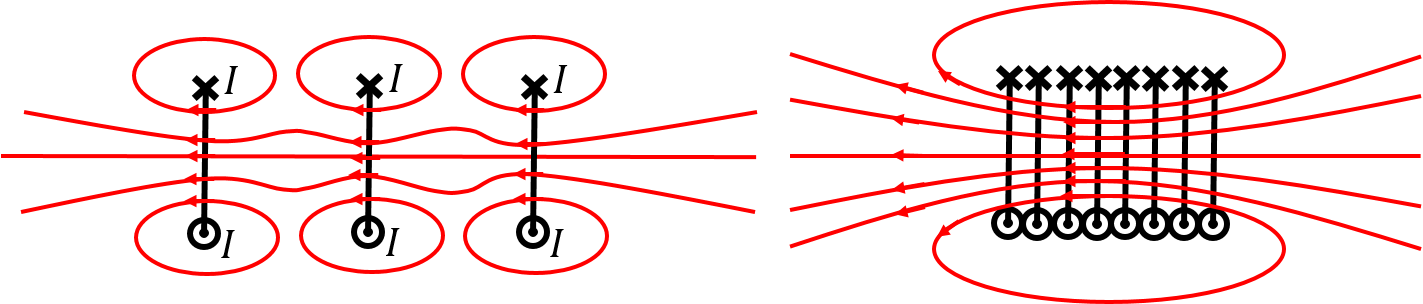
\includegraphics[width=0.8\linewidth]{files/solenoid2-611d14b5c1f0d1be219876425e557c5c.png}
\caption[]{As multiple loops of current are brought together to form a solenoid, the magnetic field inside the solenoid becomes uniform and the field outside the solenoid approaches zero.}
\label{fig:magneticsource:solenoid2}
\end{figure}

We can use Ampère's Law to determine the strength of the magnetic field inside of a solenoid, under the assumption that the magnetic field is uniform in the volume of the solenoid and zero just outside. Consider a solenoid with current, $I$, going through it, that contains $n$ loops \textit{per unit length}. In order to determine the magnetic field, $B$, inside of the solenoid, consider the rectangular Amperian loop, $abcd$, of length, $l$, illustrated in Figure~\ref{fig:magneticsource:amperesolenoid}.

\begin{figure}[!htbp]
\centering
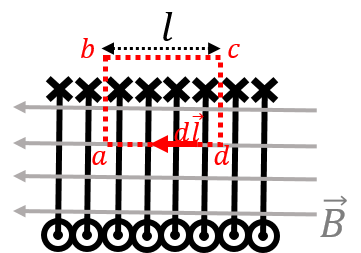
\includegraphics[width=0.4\linewidth]{files/amperesolenoid-59b241c750f8105b78b9fb29bbfc8a6b.png}
\caption[]{We use Ampère's Law with a rectangular loop to evaluate the strength of the magnetic field inside a solenoid.}
\label{fig:magneticsource:amperesolenoid}
\end{figure}

In order to evaluate the circulation of the magnetic field around the loop, $abcd$, we divide the loop up into segments, and evaluate the path integral ($\int \vec B \cdot d\vec l$) over each segment, then add those together to obtain the integral over the closed path:
\begin{equation}
\oint_{abcd} \vec B \cdot d\vec l = \int_a^b \vec B \cdot d\vec l + \int_b^c \vec B \cdot d\vec l + \int_c^d \vec B \cdot d\vec l + \int_d^a \vec B \cdot d\vec l
\end{equation}
Over each segment, the vector $d\vec l$ will be parallel to that segment. Only the last term is non-zero. The integrals over the segments $ab$ and $cd$ are zero because the magnetic field is perpendicular to $d\vec l$ over those segments (so the scalar product is zero). The integral over the segment $bc$ is zero because the magnetic field is zero just outside the solenoid. The integral over the last segment, where $d\vec l$ and $\vec B$ are parallel, is simply given by:
\begin{equation}
\oint_{abcd} \vec B \cdot d\vec l &= \int_d^a \vec B \cdot d\vec l\\
&= B \int_d^a dl\\
&= Bl
\end{equation}
since the length of the segment is $l$, and the magnetic field is constant in magnitude.

In order to apply Ampère's Law, we must determine the current that is enclosed by our Amperian loop. Since the rectangular loop has a length, $l$, it will enclose $N=nl$ loops of current, $I$, since there are $n$ loops per unit length. Thus the enclosed current is $I^{enc}=nlI$. Applying Ampère's Law, we find the magnetic field inside a solenoid:
\begin{equation}
\oint \vec B \cdot d\vec l &=\mu_0 I^{enc}\\
Bl &= \mu_0 nIl\\
\end{equation}
\begin{equation}
\therefore\;\; \boxed{B = \mu_0 nI}\quad \text{(Field inside a solenoid)}
\end{equation}
which does not depend on our (arbitrary) choice of making an Amperian loop with an arbitrary length of $l$. In practice, when solenoids are used as electromagnets, they are typically filled with a ferromagnetic material, which will magnetise when there is a current, resulting in a stronger magnetic field. This is usually done by winding a wire around an iron rod.

Note that if we extend the Amperian loop so that the bottom segment is also outside the solenoid, as in Figure~\ref{fig:magneticsource:amperesolenoid2}, it is easy to show that the magnetic field immediately outside of the solenoid must be zero. Indeed, in this case, there are an equal number of currents coming out of the page as there are going into the page, so that the net current that is enclosed by the Amperian loop (the net current that crosses the plane of the loop) is identically zero, so that the circulation must be zero, implying that the magnetic field is zero just outside the solenoid.

\begin{figure}[!htbp]
\centering
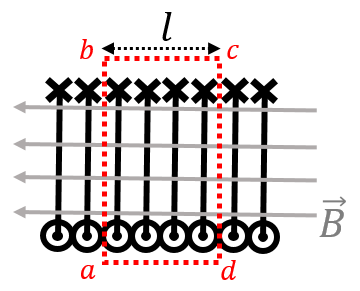
\includegraphics[width=0.4\linewidth]{files/amperesolenoid2-e48761aed6a4094ac357cc8c4af2916b.png}
\caption[]{By extending the Amperian loop to both sides of the solenoid, we conclude that the magnetic field just outside the solenoid must be zero, because the net current enclosed is zero.}
\label{fig:magneticsource:amperesolenoid2}
\end{figure}

A toroid can be thought of as a solenoid that has been bent into the shape of a circle (or rather, a torus), as illustrated in Figure~\ref{fig:magneticsource:amperetoroid}. Inside the toroid, the magnetic field forms concentric circles (not shown).

\begin{figure}[!htbp]
\centering
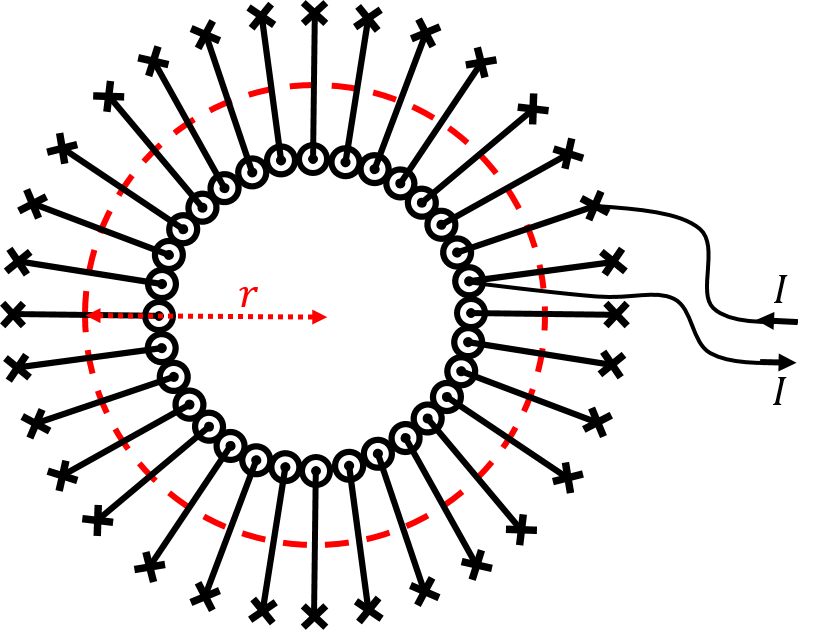
\includegraphics[width=0.6\linewidth]{files/amperetoroid-cb02fa5ffa0c5002d59a27beff662361.png}
\caption[]{An Amperian loop of radius $r$ to determine the magnetic field inside of a toroid. Note that the magnetic field everywhere outside the toroid must be zero (think of the current enclosed by Amperian loops).}
\label{fig:magneticsource:amperetoroid}
\end{figure}

Again, we can use Ampère's Law to determine the strength of the magnetic field inside the toroid. Consider the circular Amperian loop of radius $r$ that is illustrated in Figure~\ref{fig:magneticsource:amperetoroid}. Since the magnetic field is parallel to the Amperian loop everywhere along the loop, and the magnetic field does not change magnitude (by symmetry), the circulation is given by:
\begin{equation}
\oint \vec B \cdot d\vec l &= B (2\pi r)
\end{equation}
If the toroid contains $N$ loops of current, then the enclosed current is given by $I^{enc}=NI$, since the Amperian loop include $N$ times the current $I$ coming out of the page. Ampère's Law thus gives the magnitude of the magnetic field as:
\begin{equation}
\oint \vec B \cdot d\vec l &=\mu_0 I^{enc}\\
B (2\pi r) &= \mu_0 NI\\
\therefore B&=\frac{\mu_0 NI}{2\pi r}
\end{equation}
which decreases in magnitude with increasing radius, as long as we are inside the toroid. It is easy to show, by using Amperian loops that are either smaller or bigger than the toroid, that the magnetic field everywhere outside of the toroid is exactly zero (as those Amperian loops will enclose no net current). In a toroid, the magnetic field lines form closed circles. For a solenoid, there must exist a magnetic field somewhere outside the solenoid, in order for the field lines inside the solenoid to close. We can usually ignore these if the solenoid is long, as the field outside will be very weak, and very close to zero very close the solenoid (as we showed with Ampère's Law above).

\begin{framed}
\textbf{Checkpoint}\\
In Figure~\ref{fig:magneticsource:amperetoroid}, the magnetic field makes concentric circles. What direction do the field lines point?:

\begin{enumerate}
\item Clockwise.
\item Counter clockwise.
\item Upwards.
\item Not enough information to tell.
\end{enumerate}

\begin{framed}
\textbf{Answer}\\
\begin{enumerate}[resume]
\item
\end{enumerate}
\end{framed}
\end{framed}

% %%:::{tip} Checkpoint
% %%What range or position of $r$ encloses the most current in [](#fig:magneticsource:amperetoroid)?:
% %%1.  All $r$ between the $\odot$ and the $\otimes$ symbols.
% %%2.  The point directly between the $\odot$ and the $\otimes$ symbols.
% %%3.  All $r$ from the centre of the toroid to the $\odot$ symbols.
% %%4.  All $r$ beyond the $\otimes$ symbols.
% %%%	:::{tip} Answer
% %%:class: dropdown
% %%1.
% %%:::

\subsubsection{Summary}

Magnetic fields are created by moving charges. The Biot-Savart Law allows us to determine the infinitesimal magnetic field, $d\vec B$, that is produced by the current, $I$, flowing in an infinitesimal section of wire, $d\vec l$:
\begin{equation}
d\vec B = \frac{\mu_0 I}{4\pi}\frac{d\vec l\times \hat r}{r^2}
\end{equation}
where $\mu_0$ is a constant called the permeability of free space. The vector $\vec r$ points from the wire element, $d\vec l$, to the point at which we want to determine the magnetic field. In order to determine the magnetic field from a finite wire, one must sum (integrate) the contributions that come from each section of wire. It is often easier to work with the Biot-Savart law written without the unit vector, $\hat r$:
\begin{equation}
d\vec B = \frac{\mu_0 I}{4\pi}\frac{d\vec l\times \vec r}{r^3}
\end{equation}
The magnetic field at a distance, $h$, from an infinitely long wire carrying current, $I$, is given by:
\begin{equation}
B&=\frac{\mu_0 I}{2\pi h}
\end{equation}
The magnetic field from a straight current-carrying wire forms concentric circles centred around the wire. The direction of the magnetic field is given by the right-hand rule for axial vectors; with the thumb pointing in the direction of current, the fingers curl in the direction of the magnetic field.

The magnitude of the magnetic field, a distance, $h$, from the centre of a circular loop of wire with radius, $R$, carrying current, $I$, along the axis of symmetry of the loop is given by:
\begin{equation}
B=\frac{\mu_0 I}{2} \frac{R^2}{(R^2+h^2)^\frac{3}{2}}
\end{equation}
The direction of the magnetic field can also be found using the right-hand rule for axial currents. In this case, if your fingers curl in the direction of the current loop, your thumb points in the same direction as the magnetic field at the centre of the loop.

Two parallel wires carrying currents, $I_1$ and $I_2$, separated by a distance, $h$, will exert equal and opposite forces on each other with a magnitude:
\begin{equation}
F = \frac{\mu_0I_1I_2}{2\pi h}
\end{equation}
The force is attractive if the two currents flow in the same direction and repulsive otherwise.

Ampère's Law is the magnetism analogue to Gauss' Law. Just like Gauss' Law, it requires a high degree of symmetry to be applied analytically, although it is always valid. Ampère's Law relates the circulation of the magnetic field around a closed path to the current enclosed by that path:
\begin{equation}
\oint \vec B \cdot d\vec l =\mu_0 I^{enc}
\end{equation}
In order to apply Ampère's Law, we must first choose an Amperian loop over which to compute the closed path integral (instead of choosing a Gaussian surface to calculate the flux of the electric field on a closed surface). The circulation integral will be straightforward to evaluate if:

\begin{enumerate}
\item \textbf{The angle between $\vec B$ and $d\vec l$ is constant along the path}, so that:
\end{enumerate}
\begin{equation}
\oint  \vec B \cdot d\vec l &= \oint B dl \cos\theta\\
&= \cos\theta \oint B dl
\end{equation}
where $\theta$ is the angle between $\vec B$ and $d\vec l$.

\begin{enumerate}[resume]
\item \textbf{The magnitude of $\vec B$ is constant along the path}, so that:
\end{enumerate}
\begin{equation}
\cos\theta \oint B dl = B\cos\theta \oint dl
\end{equation}
The current enclosed, $I^{enc}$, corresponds to the net current that crosses the surface that is defined by the Amperian loop (a closed path always defines a surface).

Ampère's Law is straightforward to use in situations with a high degree of symmetry, such as infinitely long wires carrying current.

Solenoids are formed by combining many loops of current together, in order to form a strong and uniform magnetic field. The magnetic field inside of a solenoid has a magnitude of:
\begin{equation}
B=\mu_0nI
\end{equation}
where, $I$, is the current in the solenoid, and $n$, is the number of loops per unit length in the solenoid.  The magnetic field just outside of a solenoid is zero, and generally, the magnetic field is negligible outside of a solenoid.

A toroid is formed by bending a solenoid into a circle to form a torus. The magnetic field lines inside of a toroid form concentric circles. The magnetic field decreases with radius inside of a toroid and is identically zero everywhere outside a toroid.

\begin{framed}
\textbf{Important Equations}\\
\textbf{Biot-Savart law:}
\begin{equation}
d\vec B = \frac{\mu_0 I}{4\pi}\frac{d\vec l\times \hat r}{r^2}=\frac{\mu_0 I}{4\pi}\frac{d\vec l\times \vec r}{r^3}
\end{equation}

\textbf{Magnetic field from a finite wire:}
\begin{equation}
B = \frac{\mu_0 I}{2\pi h}
\end{equation}

\textbf{Magnetic field from an infinitely long wire:}
\begin{equation}
B = \frac{\mu_0 I}{2\pi h}
\end{equation}

\textbf{Magnetic field from a circular loop of current:}
\begin{equation}
B=\frac{\mu_0 I}{2} \frac{R^2}{(R^2+h^2)^\frac{3}{2}}
\end{equation}

\textbf{Force between two wires:}
\begin{equation}
F = \frac{\mu_0I_1I_2}{2\pi h}
\end{equation}

\textbf{Ampère's law:}
\begin{equation}
\oint \vec B \cdot d\vec l =\mu_0 I^{enc}
\end{equation}
\end{framed}

\subsubsection{Thinking about the material}

\begin{framed}
\textbf{Reflect and research}\\
\begin{itemize}
\item Who discovered Ampère's Law? What did Ampère discover?
\item What are three common uses of electromagnets.
\item How does a coil gun work?
\end{itemize}
\end{framed}

\begin{framed}
\textbf{To try at home}\\
\begin{itemize}
\item Use a battery and some wire to build an electromagnet. Is it stronger if you use a ferromagnetic core?
\item Research the current that your household electronics have. Are design choices affected by the magnetic fields generated by the current in these electronics?
\end{itemize}
\end{framed}

\begin{framed}
\textbf{To try in the lab}\\
\begin{itemize}
\item (Simulation) Calculate the magnetic field from a loop of current at all positions in space (not only on the axis of symmetry).
\item Propose an experiment to characterize the magnetic field produced by Helmholtz coils.
\item Propose an experiment to build and test a coil gun.
\end{itemize}
\end{framed}

\subsubsection{Sample problems and solutions}

\paragraph{Problems}

\begin{framed}
\textbf{Problem 21.1}\\
A square loop of wire with side length, $L$, carries current, $I$, as shown in Figure~\ref{fig:magneticsource:squareloop}. What is the magnetic field at the centre of the loop?

\begin{figure}[!htbp]
\centering
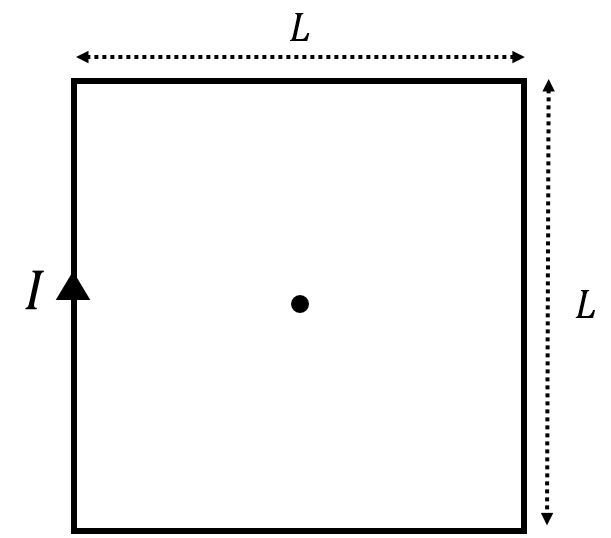
\includegraphics[width=0.3\linewidth]{files/squareloop-b9f08214664e39de556569ccfa71efa9.png}
\caption[]{A square loop of current.}
\label{fig:magneticsource:squareloop}
\end{figure}
\end{framed}

\begin{framed}
\textbf{Problem 21.2}\\
Helmholtz coils are an arrangement of two parallel loops of current that produce a nearly uniform magnetic field. Helmholtz coils are formed by two identical circular loops of radius $R$, carrying the same current, $I$, where the centres of the coils are separated by a distance, $R$, as illustrated in Figure~\ref{fig:magneticsource:helmholtzdiagram}. Determine the magnetic field as a function of $z$, along the axis of symmetry of the coils, where the origin is located half way between the two coils. Make a plot of the magnetic field as a function of $z$ from each coil, as well as the total magnetic field to show that it is close to uniform between the coils.

\begin{figure}[!htbp]
\centering
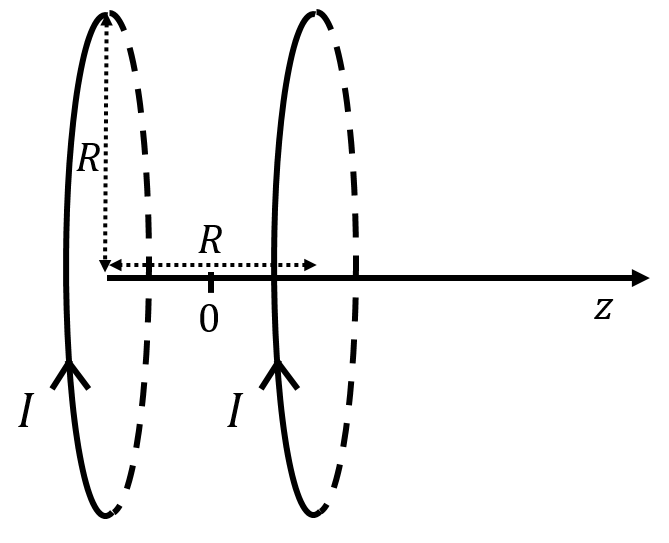
\includegraphics[width=0.4\linewidth]{files/helmholtzdiagram-5e71f8519586a40e19b5c4bd4c183262.png}
\caption[]{A Helmholtz coil arrangement.}
\label{fig:magneticsource:helmholtzdiagram}
\end{figure}
\end{framed}

\paragraph{Solutions}

\begin{framed}
\textbf{Solution 21.1}\\
The square loop is simply made of four straight sections of wire of length, $L$. The magnetic field from each section of wire is into the page, which you can easily verify with your right-hand (with your thumb in the direction of current, your fingers curl in the direction of the resulting magnetic field).

The magnetic field at the centre is just four times the magnetic field produced by a single segment, which we determined in this chapter. The magnetic field at the centre of the loop is thus four times the magnetic field at a distance, $h=\frac{L}{2}$, from a wire of length, $L$:
\begin{equation}
B &= 4\times\frac{\mu_0 I}{2\pi \frac{L}{2}}\frac{L/2}{\sqrt{\frac{L^2}{4}+\frac{L^2}{4}}}=2\sqrt 2\frac{\mu_0 I}{\pi L}
\end{equation}
\end{framed}

\begin{framed}
\textbf{Solution 21.2}\\
We know that the magnetic field at a distance, $h$, from the centre of a loop of current, along its axis of symmetry is given by:
\begin{equation}
 B(h) = \frac{\mu_0 I}{2}\frac{R^2}{(R^2+h^2)^{\frac{3}{2}}}
\end{equation}
For the two coils in the Helmholtz configuration, the magnetic field from each coil will be in the same direction. The centre of the two coils are located at $z=\pm\frac{R}{2}$. Thus, if we are located at position, $z$, along the $z$ axis, one coil will be at a distance of $z+\frac{R}{2}$, and the other at a distance $z -\frac{R}{2}$. The total magnetic field as a function of $z$ is then given by:
\begin{equation}
B^{tot}(z) &= B\left(z+\frac{R}{2}\right)+B\left(z-\frac{R}{2}\right)\\
&=\frac{\mu_0 I}{2}\frac{R^2}{(R^2+\left(z+\frac{R}{2}\right)^2)^{\frac{3}{2}}}+\frac{\mu_0 I}{2}\frac{R^2}{(R^2+\left(z-\frac{R}{2}\right)^2)^{\frac{3}{2}}}
\end{equation}
We can plot this function, as well as the two individual terms using python. For information, we show the code below. In order to make the plot, we need to choose some reasonable values for the radius of the coils and the current through the coils, for example:

\begin{itemize}
\item $R=0.3 {\rm m}$
\item $I=0.5 {\rm A}$
\end{itemize}

\begin{verbatim}
#Import the modules that we need:
import numpy as np
import matplotlib.pyplot as plt

#Define some constants:
mu0 = 4*np.pi*1e -7 #4 pi 
I = 0.5
R = 0.3

#Define the values on the z axis, from -2R to +2R, in 100 increments
z = np.linspace( -2*R,2*R,100)

#Determine the magnetic field from the coils at those values of z
#The coil at z = - R/2:
B1 = (mu0*I)/2 * R**2/((R**2+(z+R/2)**2)**(3/2))
#The coil at z = + R/2:
B2 = (mu0*I)/2 * R**2/((R**2+(z -R/2)**2)**(3/2))
#The sum:
B = B1 + B2

#Make the plot
plt.figure(figsize=(10,6))
plt.plot(z,B1,label='Coil at z= -R/2')
plt.plot(z,B2,label='Coil at z=+R/2')
plt.plot(z,B,label='Total')
plt.legend()
plt.xlabel('z position [m]')
plt.ylabel('Magnetic field [T]')
plt.show()
\end{verbatim}

\begin{figure}[!htbp]
\centering
\begin{quote}
\begin{figure}[!htbp]
\centering
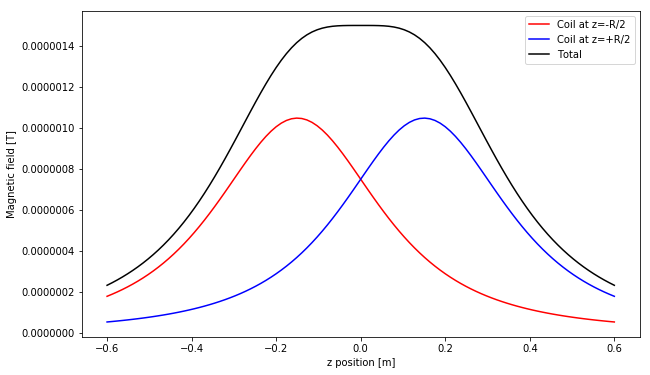
\includegraphics[width=0.8\linewidth]{files/helmholtzcoil-179de3570ec926b3e29eaadde6cb1a4b.png}
\caption[]{Magnetic field from each coil, as well as their sum, for two coils in the Helmholtz configuration}
\label{fig:magneticsource:helmholtzcoil}
\end{figure}

As advertised, we see a region between the Helmholtz coils where the magnetic field is nearly uniform.
\end{quote}
\end{figure}
\end{framed}